% PTE Core 模考 43B —— 口语 错题与详解·整理卷  版本 000（自包含）
% 编译: xelatex 本文件.tex   （需 Noto CJK + TeX Gyre Heros 字体）
% 本版本含图片，依赖同目录的 img/ 子目录。
\documentclass[11pt]{article}

% --------- 样式（原 ptestyle.sty，已内联）---------
% ============================================================
%  ptestyle.sty  —  PTE 模考错题整理卷 共享样式
%  编译引擎: XeLaTeX  (中英混排, 需要 Noto CJK 字体)
% ============================================================

\usepackage[a4paper,margin=2cm,headsep=4mm]{geometry}
\usepackage{fontspec}
\usepackage{xeCJK}
\usepackage[table]{xcolor}
\usepackage[normalem]{ulem}        % \sout 删除线
\usepackage{tabularx}
\usepackage{array}
\usepackage{ragged2e}
\usepackage{enumitem}
\usepackage[most]{tcolorbox}
\usepackage{fancyhdr}
\usepackage{graphicx}
\usepackage{pifont}                % \ding{51}=✓ \ding{55}=✗（阅读对错标注）
\usepackage{needspace}
\usepackage{tikz}

% ---------- 字体 ----------
\setmainfont{TeX Gyre Heros}            % 拉丁: Helvetica 风格(纤细清晰)
\setCJKmainfont{Noto Sans CJK SC}
\setCJKsansfont{Noto Sans CJK SC}
\newfontfamily\cjkserif{Noto Serif CJK SC}
\linespread{1.18}
\setlength{\parindent}{0pt}
\setlength{\parskip}{4pt}

% ---------- 配色 ----------
\definecolor{cWrong}{HTML}{D32F2F}     % 红  = 修改 / 错误
\definecolor{cFix}{HTML}{1B7F3B}       % 绿  = 正确建议
\definecolor{cDelete}{HTML}{1565C0}    % 蓝  = 删除
\definecolor{cInsert}{HTML}{7B1FA2}    % 紫  = 插入
\definecolor{cPartial}{HTML}{E07B00}   % 橙  = 部分得分
\definecolor{cNote}{HTML}{0277BD}      % 蓝  = 注解
\definecolor{cAccent}{HTML}{16A085}    % 主题青绿(平台主色)
\definecolor{cWrongBg}{HTML}{FBE0E0}
\definecolor{cDelBg}{HTML}{DCE8FB}
\definecolor{cInsBg}{HTML}{EEE0F5}
\definecolor{cHead}{HTML}{20303A}
\definecolor{cGrayBox}{HTML}{F4F6F7}
\definecolor{cModelBg}{HTML}{EAF7EF}
\definecolor{cYouBg}{HTML}{FFF7F5}
\definecolor{cNoteBg}{HTML}{EAF3FA}
\definecolor{cRule}{HTML}{D7DEE2}

% ---------- 行内批改宏 (复刻平台标注) ----------
% \fix{原词}{正确}  红色删除线 + 绿色上标改正  (修改/拼写/空格)
\newcommand{\fix}[2]{%
  \colorbox{cWrongBg}{\textcolor{cWrong}{\sout{#1}}}%
  \,\textsuperscript{\textcolor{cFix}{\footnotesize #2}}}
% \del{原词}  蓝色删除线  (应删除)
\newcommand{\del}[1]{%
  \colorbox{cDelBg}{\textcolor{cDelete}{\sout{#1}}}%
  \,\textsuperscript{\textcolor{cDelete}{\footnotesize 删}}}
% \ins{词}  紫色下划线  (应插入)
\newcommand{\ins}[1]{%
  \textsuperscript{\textcolor{cInsert}{\footnotesize $\wedge$}}%
  \colorbox{cInsBg}{\textcolor{cInsert}{#1}}}
% \miss{词}  灰色删除线  (口语漏读 / 未作答)
\newcommand{\miss}[1]{\textcolor{gray}{\sout{#1}}}
% \add{原词}{改正}  橙色波浪线 + "补"标签  (平台漏标、本卷补标的错误)
\definecolor{cAdd}{HTML}{E65100}
\newcommand{\add}[2]{%
  \textcolor{cAdd}{\uwave{#1}}%
  \,\textsuperscript{\textcolor{cAdd}{\footnotesize 补：#2}}}
% 高亮(口语发音): 好/中/差
\newcommand{\spk}[2]{\textcolor{#1}{#2}}

% ---------- 评分单元格着色 ----------
\newcommand{\sfull}[1]{\textcolor{cFix}{\bfseries #1}}     % 满分
\newcommand{\spart}[1]{\textcolor{cPartial}{\bfseries #1}} % 部分
\newcommand{\szero}[1]{\textcolor{cWrong}{\bfseries #1}}   % 零/低分

% ---------- 分数小标签 ----------
\newtcbox{\chip}[1][cAccent]{on line, boxsep=2pt, left=4pt, right=4pt, top=1pt,
  bottom=1pt, arc=3pt, colback=#1, colframe=#1, coltext=white, nobeforeafter,
  fontupper=\bfseries\footnotesize}

% ---------- 题块小标题 ----------
\newcommand{\ptesub}[1]{%
  \par\needspace{2\baselineskip}\smallskip
  {\color{cAccent}\rule[-0.2ex]{3pt}{1.05em}}\hspace{6pt}%
  {\bfseries\color{cHead}#1}\par\nopagebreak\smallskip}

% ---------- 题块外框 ----------
% \begin{qblock}{标号·题型}{右上信息(得分/用时)} ... \end{qblock}
\newtcolorbox{qblock}[2]{
  breakable, enhanced, arc=2.5pt,
  colback=white, colframe=cRule, boxrule=0.6pt,
  left=11pt, right=11pt, top=8pt, bottom=10pt,
  toptitle=3pt, bottomtitle=3pt, lefttitle=11pt, righttitle=11pt,
  colbacktitle=cHead, coltitle=white, fonttitle=\bfseries,
  title={#1\hfill\normalfont\bfseries\small #2}}

% ---------- 文本块: 题干 / 范文 / 你的作答 / 建议 ----------
\newtcolorbox{promptbox}{enhanced, breakable, colback=cGrayBox, colframe=cGrayBox,
  arc=2pt, left=8pt, right=8pt, top=6pt, bottom=6pt, boxrule=0pt}
\newtcolorbox{modelbox}{enhanced, breakable, colback=cModelBg, colframe=cModelBg,
  borderline west={3pt}{0pt}{cFix}, arc=1pt, left=8pt, right=8pt, top=6pt, bottom=6pt, boxrule=0pt}
\newtcolorbox{youbox}{enhanced, breakable, colback=cYouBg, colframe=cYouBg,
  borderline west={3pt}{0pt}{cWrong}, arc=1pt, left=8pt, right=8pt, top=6pt, bottom=6pt, boxrule=0pt}
\newtcolorbox{notebox}{enhanced, breakable, colback=cNoteBg, colframe=cNoteBg,
  borderline west={3pt}{0pt}{cNote}, arc=1pt, left=8pt, right=8pt, top=6pt, bottom=6pt, boxrule=0pt}

% ---------- 评分表 ----------
% 用法见正文; 这里给表头宏
\newcommand{\scorehead}{%
  \rowcolors{2}{cGrayBox}{white}
  \arrayrulecolor{cRule}}

% ---------- 章节大标题 ----------
\newcommand{\ptesection}[3]{% #1=中文名 #2=英文名 #3=该项分数
  \addcontentsline{toc}{section}{#1}%
  \needspace{6\baselineskip}
  \begin{tcolorbox}[enhanced, colback=cAccent, colframe=cAccent, sharp corners,
     left=14pt, right=14pt, top=10pt, bottom=10pt, boxrule=0pt]
    {\fontsize{20}{24}\selectfont\bfseries\color{white} #1\ \ }%
    {\large\color{white!85} #2}\hfill
    {\large\color{white}本项得分\ \ }{\fontsize{22}{24}\selectfont\bfseries\color{white} #3}%
    \ {\color{white!85}/ 90}
  \end{tcolorbox}}

% ---------- 题型小节分隔 (口语 RA/RS/DI/RTS/ASQ 等) ----------
\newcommand{\ptetask}[2]{%
  \addcontentsline{toc}{subsection}{#1\ #2}%
  \needspace{4\baselineskip}\medskip
  \begin{tcolorbox}[enhanced, colback=cHead, colframe=cHead, sharp corners,
     left=12pt, right=12pt, top=5pt, bottom=5pt, boxrule=0pt]
    {\large\bfseries\color{white} #1}\ \ {\color{white!80} #2}
  \end{tcolorbox}\smallskip}

% ---------- 口语 AI 语音识别着色 (复刻平台: 优/良/差 + 停顿) ----------
\definecolor{cSpkGood}{HTML}{2E9E5B}   % 优 绿
\definecolor{cSpkOk}{HTML}{C77F00}     % 良 黄/琥珀
\definecolor{cSpkBad}{HTML}{E0352B}    % 差 红
\newcommand{\sg}[1]{\textcolor{cSpkGood}{#1}}   % 优
\newcommand{\sy}[1]{\textcolor{cSpkOk}{#1}}     % 良
\newcommand{\sr}[1]{\textcolor{cSpkBad}{#1}}    % 差
\newcommand{\smiss}[1]{\textcolor{cSpkBad}{\sout{#1}}}  % 漏读 (红删除线)
\newcommand{\pse}{{\color{gray}\,/\,}}          % 停顿
\newcommand{\asrlegend}{{\footnotesize\color{gray}AI 语音识别\quad
  {\color{cSpkGood}\textbullet}\,优\ \ {\color{cSpkOk}\textbullet}\,良\ \
  {\color{cSpkBad}\textbullet}\,差\ \ {\color{gray}/}\,停顿\ \
  {\color{cSpkBad}\sout{词}}\,漏读}}
\newtcolorbox{asrbox}{enhanced, breakable, colback=white, colframe=cRule,
  boxrule=0.6pt, arc=1pt, left=8pt, right=8pt, top=6pt, bottom=6pt}

% ---------- 中文翻译行 ----------
\newcommand{\zh}[1]{{\footnotesize\textcolor{cNote}{\textbf{译}}\ \textcolor{gray}{#1}}}

% ---------- 阅读填空 / 选择 对错标注 ----------
\newcommand{\rok}[1]{{\color{cFix}\ding{51}\,#1}}                 % 选对(绿勾 + 词)
\newcommand{\rno}[2]{{\color{cWrong}\ding{55}\,\sout{#1}}\,{\footnotesize\color{cFix}(答案:\,#2)}}  % 选错: 你的(红删) + (答案:正确)
\newcommand{\rblank}[1]{{\color{cFix}\underline{\,#1\,}}}         % 直接给空的正确答案(无你的作答时)

% ---------- 听力专用 ----------
\newcommand{\hiw}[2]{{\color{cWrong}\uline{#1}}\,{\footnotesize\color{cFix}(听:#2)}} % HIW: 屏幕错词(红下划线)+ 实际读音
\newcommand{\lhit}[1]{{\color{cFix}#1}}                           % WFD: 命中的词(绿)
\newcommand{\lmiss}[1]{{\color{cWrong}\sout{#1}}}                 % WFD: 多余/错误的词(红删, 1B 配色)
% ---- WFD 逐词批改 · 本套 2B 平台配色（与 1B 相反）：绿=命中 / 红括号=漏写 / 灰删除线=多写或听错 ----
% 说明: 2B 平台把"漏写"标红(加括号)、"多写/听错"标灰删除线; 本卷忠于原图按此复刻。
\newcommand{\womit}[1]{{\color{cWrong}(#1)}}                      % WFD: 漏写(正确答案有、你没写)——红色括号
\newcommand{\wbad}[1]{{\color{gray}\sout{#1}}}                    % WFD: 多写/听错(你写了但错)——灰删除线
\newcommand{\wfdlegend}{{\footnotesize\color{gray}WFD 配色：\
  {\color{cFix}命中}\ \ {\color{cWrong}(漏写)}\ \ {\color{gray}\sout{多写/听错}}}}

% ---------- 颜色图例 ----------
\newcommand{\ptelegend}{%
  \begin{tcolorbox}[enhanced, colback=cGrayBox, colframe=cRule, boxrule=0.5pt,
    arc=2pt, left=10pt, right=10pt, top=6pt, bottom=6pt]
  {\bfseries\color{cHead}颜色说明\quad}
  \fix{改}{正}~修改/拼写\quad
  \del{删}~应删除\quad
  \ins{插}~应插入\quad
  \add{补}{改正}~平台漏标(本卷补标)\quad
  {\color{cFix}\rule{1em}{0.6em}}~范文/正确\quad
  {\color{cNote}\rule{1em}{0.6em}}~AI 建议
  \end{tcolorbox}}

% ---------- 页眉页脚 ----------
\pagestyle{fancy}
\fancyhf{}
\renewcommand{\headrulewidth}{0.4pt}
\renewcommand{\footrulewidth}{0pt}
\fancyhead[L]{\footnotesize\color{cHead}\bfseries PTE Core 模考 43B}
\fancyhead[R]{\footnotesize\color{gray} 错题与详解整理卷}
\fancyfoot[C]{\footnotesize\color{gray}\thepage}

\begin{document}

% --------- 封面（原 cover.tex）---------
% ---------- 封面 / 成绩总览 ----------
\definecolor{mListen}{HTML}{1F3A5F}
\definecolor{mRead}{HTML}{C2D70B}
\definecolor{mSpeak}{HTML}{4D4D4D}
\definecolor{mWrite}{HTML}{A01B7D}

\begin{titlepage}
\thispagestyle{empty}
\centering
\vspace*{1.4cm}

{\fontsize{30}{36}\selectfont\bfseries\color{cHead} PTE Core 模考 43B}\\[4mm]
{\fontsize{17}{20}\selectfont\color{cAccent}\bfseries 错题与详解 · 整理卷}\\[3mm]
{\color{gray} APEUni / 猩际 完整模考 43B（8.7 新考试版本）　·　提交时间 2026-07-03 17:45}\\[1.2cm]

% ---- 总分 ----
\begin{tcolorbox}[width=0.62\textwidth, halign=center, enhanced,
  colback=cAccent, colframe=cAccent, arc=6pt, boxrule=0pt, top=10pt, bottom=10pt]
  {\color{white}\large 总分 Overall}\\[2pt]
  {\fontsize{46}{50}\selectfont\bfseries\color{white} 29}
\end{tcolorbox}

\vspace{1.0cm}

% ---- 四项分数条形图（条长 = 得分 / 90，比例 1pt = 1/9 cm）----
\begin{tcolorbox}[width=0.84\textwidth, enhanced, colback=white, colframe=cRule,
  boxrule=0.8pt, arc=4pt, left=18pt, right=18pt, top=14pt, bottom=14pt]
\setlength{\tabcolsep}{6pt}\renewcommand{\arraystretch}{1.7}
\sffamily
\begin{tabular}{@{}r@{\hskip 8pt}l@{\hskip 10pt}l@{}}
 \bfseries Listening 听力 & {\color{mListen}\rule{3.56cm}{0.42cm}} & {\bfseries\large 32}\\
 \bfseries Reading 阅读   & {\color{mRead}\rule{5.67cm}{0.42cm}}   & {\bfseries\large 51}\\
 \bfseries Speaking 口语  & {\color{mSpeak}\rule{1.33cm}{0.42cm}}  & {\bfseries\large 12}\\
 \bfseries Writing 写作   & {\color{mWrite}\rule{2.33cm}{0.42cm}}  & {\bfseries\large 21}\\
\end{tabular}\\[2mm]
{\footnotesize\color{gray} 满分 90　|　刻度: 条长 = 得分 / 90}
\end{tcolorbox}

\vspace{0.8cm}

% ---- 本卷收录范围 ----
\begin{tcolorbox}[width=0.84\textwidth, enhanced, colback=cModelBg, colframe=cFix,
  boxrule=0pt, borderline west={3pt}{0pt}{cFix}, arc=3pt, left=14pt, right=14pt, top=8pt, bottom=8pt]
{\bfseries\color{cHead}本卷收录}\quad{\small 本次只做了\textbf{阅读}与\textbf{听力}，另收录口语的 \textbf{DI 看图说话}题；
共 \textbf{阅读 15 题 · 听力 15 题 · 口语 DI 5 题}。写作及口语其它题型（RA/RS/RTS/ASQ 等）未收录。}
\end{tcolorbox}

\vfill
\begin{flushleft}\small\color{gray}
\textbf{说明:}本卷由本次模考的题目与"答案 \& 解析"截图逐题誊写、重新排版而成,完整保留每道题的
\emph{题干 / 原文、选项 / 词库、你的作答、正确答案、平台中文解析与逐项得分}。\\
所有对错按平台标注用颜色标出(\rok{绿勾}=选对; {\color{cWrong}\ding{55}}\,红叉=选错并给出正确答案)。原始截图不可复制、仅能看图,本卷内容均为人工对照誊录,若与原图有出入以原图为准。
\emph{个别题(阅读 R01 选项 3--5、R14 选项 A)在原图中被平台悬浮条遮挡,已照实标注。}
\end{flushleft}
\vspace{4mm}
\ptelegend
\end{titlepage}

% --------- 口语正文（原 sec_speaking_body.tex）---------
% ===================== 口语 Speaking（仅收录 DI 看图说话）=====================
\ptesection{口语}{Speaking · DI 看图说话（本卷仅收录 DI）}{12}

\vspace{1mm}
{\small\color{gray} 本次仅收录口语中的\textbf{看图说话（Describe Image, DI）5 题}；朗读、复述句子、情景应答、简短回答等其它口语题型未收录。
每题保留\textbf{配图}、你的\textbf{作答文字稿（语音识别 ASR）}、录音与平台\textbf{总分}。
\textbf{注意}：本套平台"答案 \& 评分详情"截图里，DI 只给出\textbf{合并总分}（如 10/90），未展开 Content／Pronunciation／Fluency 逐项分，也未提供参考范文；本卷据实收录，未展开的部分留待平台补充。口语总分 \textbf{12 / 90}（含本卷未收录的其它题型）。}
\vspace{2mm}

% ---------------- Q1 ----------------
\begin{qblock}{DI\,1\quad DI \#1189\ \ Pet Services}{描述图 · 总分 \textcolor{cAccent}{\bfseries 10 / 90}}
\ptesub{配图 Image（饼图 Pie Chart）}
\begin{center}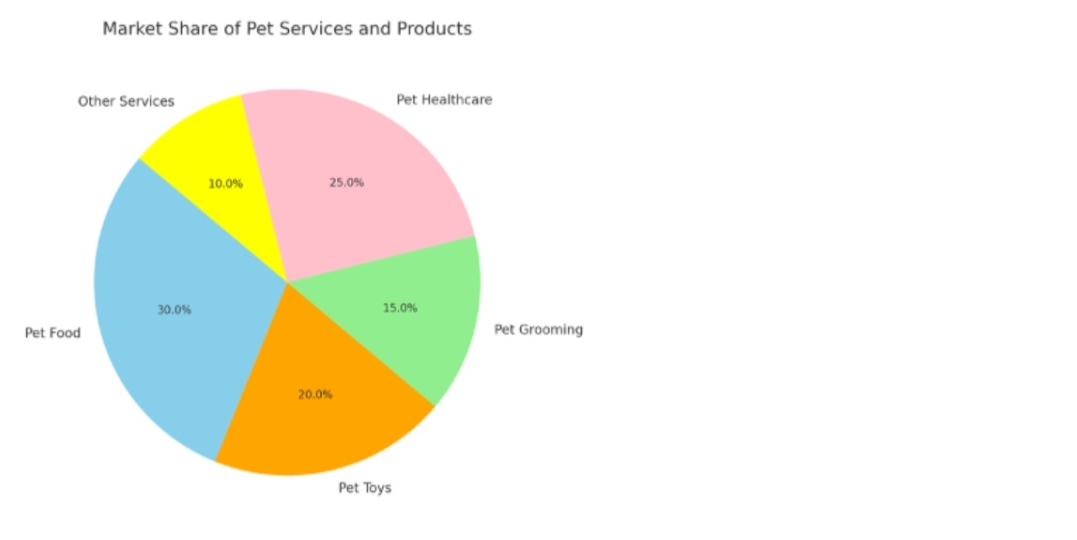
\includegraphics[width=0.86\linewidth]{img/di_pet_services.png}\end{center}
\ptesub{你的作答（语音识别文字稿 ASR Transcript）}
\begin{asrbox}
This pie chart gives information about market share of pet services and products. From the picture we can see in pet grooming the value is 15 percent. In pet toys the proportion is higher, which is 20 percent. The highest number is in pet food, around 30 percent. And the lowest percentage is in other services, just 10 percent. To sum up, the graph tells about pet services and products.
\end{asrbox}
\zh{这张饼图给出的是宠物服务与产品市场份额的信息。从图中可以看到，宠物美容的占比是 15\%；宠物玩具的比例更高，为 20\%；最高的是宠物食品，约 30\%；最低的是其它服务，只有 10\%。总的来说，这张图讲的是宠物服务与产品。}
{\footnotesize\color{gray}（注：作答漏提了 Pet Healthcare 25\% 这一类别，原图饼图共 5 类：Pet Healthcare 25\%、Pet Grooming 15\%、Pet Toys 20\%、Pet Food 30\%、Other Services 10\%。）}
\smallskip
\textbf{总分：}\ {\color{cAccent}\bfseries 10 / 90}\quad{\footnotesize\color{gray}（DI CN V4.0；录音 0:35，用时 01:01）}
\end{qblock}

% ---------------- Q2 ----------------
\begin{qblock}{DI\,2\quad DI \#1186\ \ Estate Sales}{描述图 · 总分 \textcolor{cAccent}{\bfseries 10 / 90}}
\ptesub{配图 Image（柱状图 Bar Chart）}
\begin{center}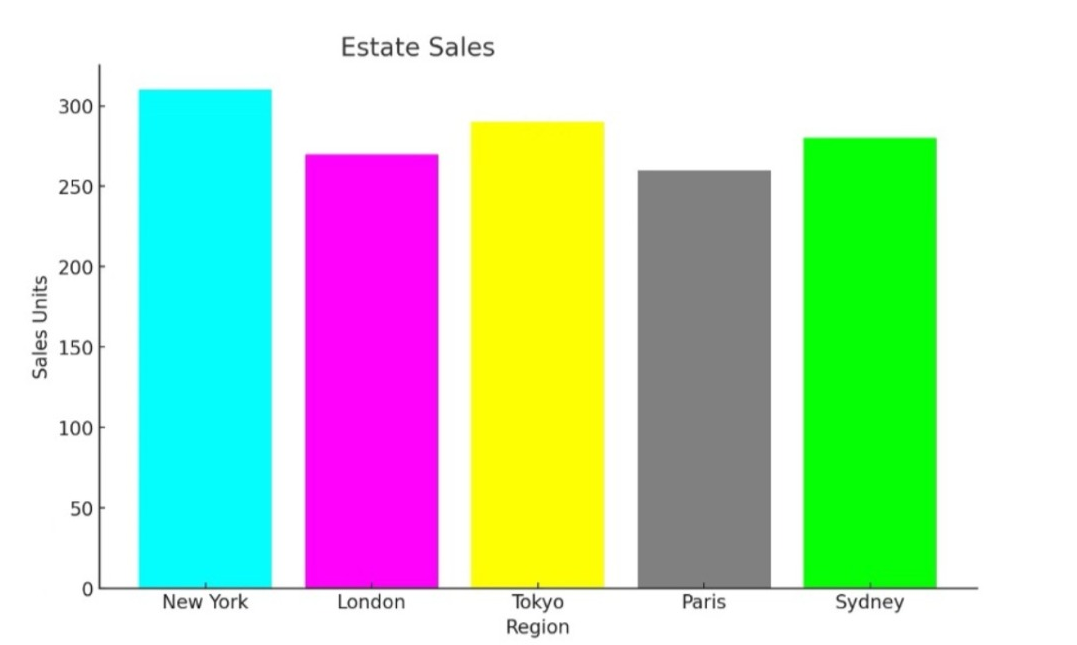
\includegraphics[width=0.86\linewidth]{img/di_estate_sales.png}\end{center}
\ptesub{你的作答（语音识别文字稿 ASR Transcript）}
\begin{asrbox}
This bar chart gives information about estate sales. From the picture we can see in London the value is 260. In Tokyo the number is higher, which is 275. The highest one is in New York, around 310. And the lowest point is in Paris, just 250. To sum up, the graph tells about estate sales.
\end{asrbox}
\zh{这张柱状图给出的是房产销售情况的信息。从图中可以看到，伦敦的数值是 260；东京更高，为 275；最高的是纽约，约 310；最低的是巴黎，只有 250。总的来说，这张图讲的是房产销售情况。}
{\footnotesize\color{gray}（注：作答漏提了 Sydney 这一城市；口述的数值与图中读数略有出入（图中约为 New York 310 / London 270 / Tokyo 290 / Paris 260 / Sydney 280），以图为准。）}
\smallskip
\textbf{总分：}\ {\color{cAccent}\bfseries 10 / 90}\quad{\footnotesize\color{gray}（DI CN V4.0；录音 0:28，用时 00:54）}
\end{qblock}

% ---------------- Q3 ----------------
\begin{qblock}{DI\,3\quad DI \#1148\ \ Electricity Usage}{描述图 · 总分 \textcolor{cAccent}{\bfseries 10 / 90}}
\ptesub{配图 Image（折线图 Line Chart）}
\begin{center}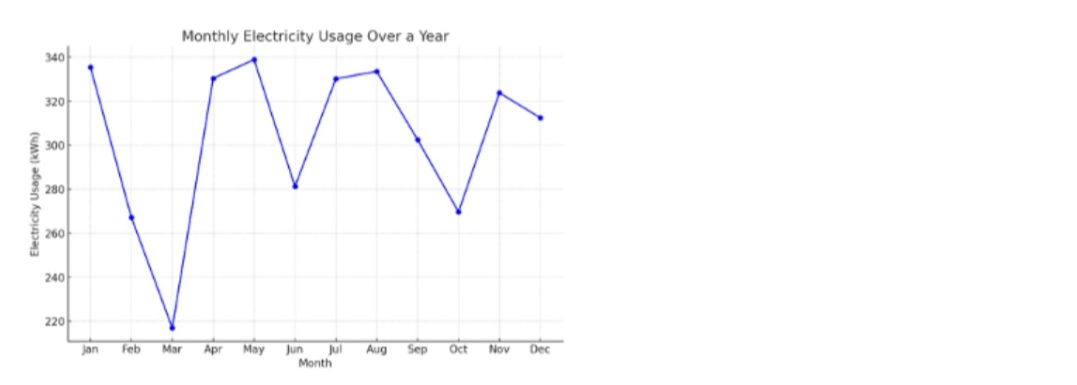
\includegraphics[width=0.86\linewidth]{img/di_electricity_usage.png}\end{center}
\ptesub{你的作答（语音识别文字稿 ASR Transcript）}
\begin{asrbox}
This line chart gives information about monthly electricity usage over a year. From the picture we can see in June the value is 280. In July the number is higher, which is 330. The highest usage is in May, around 340. And the lowest one is in March, just 210. There are many other months, such as August, October and December. To sum up, the graph tells about monthly electricity usage.
\end{asrbox}
\zh{这张折线图给出的是一年中每月用电量的信息。从图中可以看到，六月的数值是 280；七月更高，为 330；最高的是五月，约 340；最低的是三月，只有 210；还有其它一些月份，比如八月、十月和十二月。总的来说，这张图讲的是每月用电量。}
\smallskip
\textbf{总分：}\ {\color{cAccent}\bfseries 10 / 90}\quad{\footnotesize\color{gray}（DI CN V4.0；录音 0:35，用时 01:02）}
\end{qblock}

% ---------------- Q4 ----------------
\begin{qblock}{DI\,4\quad DI \#949\ \ Crop Distribution}{描述图 · 总分 \textcolor{cAccent}{\bfseries 10 / 90}}
\ptesub{配图 Image（世界地图 World Map）}
\begin{center}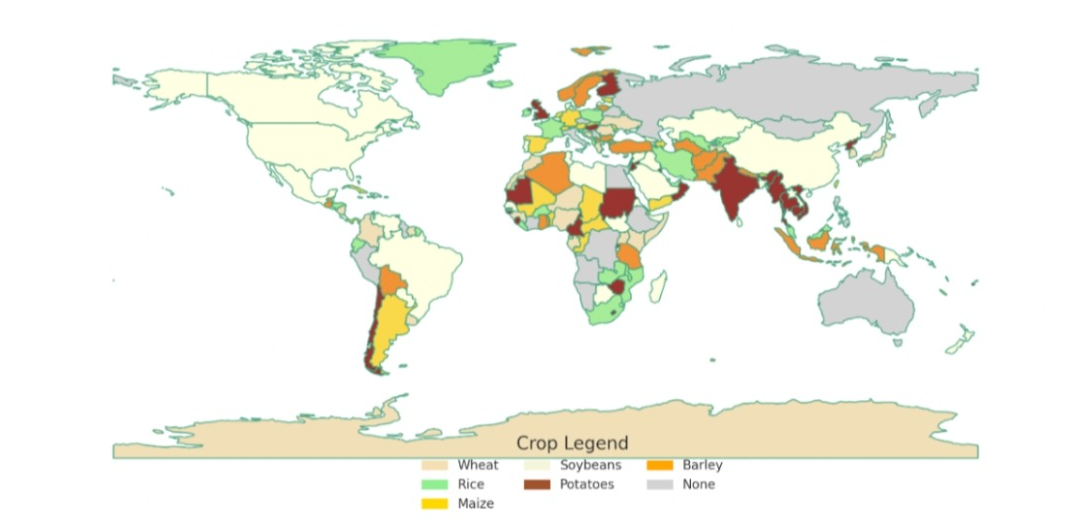
\includegraphics[width=0.9\linewidth]{img/di_crop_distribution.png}\end{center}
\ptesub{你的作答（语音识别文字稿 ASR Transcript）}
\begin{asrbox}
The following graph gives information about the distribution of crops across the world. According to the picture, I can see the geographical locations where crops are predominantly grown. From the picture, in China and North America soybeans are the main agricultural products. Moreover, there are some regions like Russia and Austria with no crop. Lastly, maize is grown in South America. To sum up, the graph tells about distribution of crops.
\end{asrbox}
\zh{这张图给出的是全球作物分布的信息。从图中可以看出作物主要种植的地理位置。从图中看，中国和北美地区大豆是主要农产品；此外，像俄罗斯和奥地利这样的一些地区没有作物；最后，南美洲种植玉米。总的来说，这张图讲的是作物分布情况。}
{\footnotesize\color{gray}（注：口述"Austria"应为"Australia"（澳大利亚，图中该区域标为 None）；图例另有 Wheat / Rice / Barley / Potatoes 类别，作答未逐一提及。）}
\smallskip
\textbf{总分：}\ {\color{cAccent}\bfseries 10 / 90}\quad{\footnotesize\color{gray}（DI CN V4.0；录音 0:39，用时 01:05）}
\end{qblock}

% ---------------- Q5 ----------------
\begin{qblock}{DI\,5\quad DI \#1160\ \ Riverside Town}{描述图 · 总分 \textcolor{cAccent}{\bfseries 10 / 90}}
\ptesub{配图 Image（照片 Photo）}
\begin{center}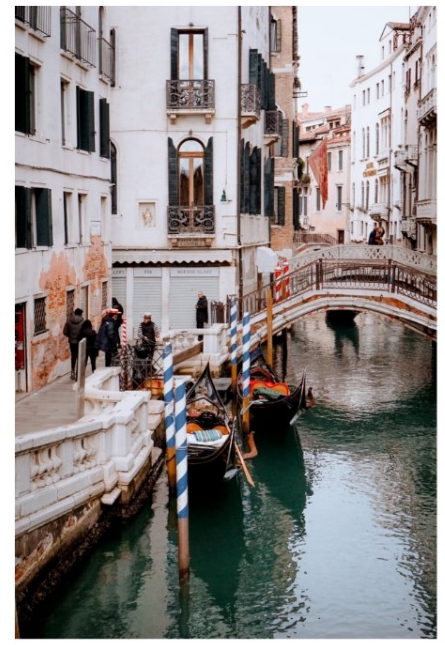
\includegraphics[width=0.55\linewidth]{img/di_riverside_town.png}\end{center}
\ptesub{你的作答（语音识别文字稿 ASR Transcript）}
\begin{asrbox}
The picture gives information about a riverside town. There is a small river in the picture, with an arch bridge over the river. From the picture we can see some small boat in the river, two of which are moored to the bank, one of which is sailing across the bridge. Some tourists are on the bank, seeming to be interested by the boats. On the both banks, a lot of four-storyed buildings are very close to the river. To sum up, the graph tells about a riverside town.
\end{asrbox}
\zh{这张图给出的是一个河边小镇的信息。图中有一条小河，河上有一座拱桥。从图中可以看到河里有几只小船，其中两只停靠在岸边，一只正驶过桥下。岸边有些游客，似乎对这些船很感兴趣。两岸有许多四层楼高的建筑，紧邻河边。总的来说，这张图讲的是一个河边小镇。}
\smallskip
\textbf{总分：}\ {\color{cAccent}\bfseries 10 / 90}\quad{\footnotesize\color{gray}（DI CN V4.0；录音 0:15，用时 00:41）}
\end{qblock}

\end{document}
